\section{Evaluation}\label{sec:experiments}
In our experimental evaluation, we study the effect of batching at the storage and the validator, the performance of our validator reordering algorithms and policies, and the impact of system configuration parameters. In particular, we asked the following questions:
\begin{enumerate}
\item\vspace{-.5em} How well do our validator reordering algorithms from Section~\ref{subsec:validator_reordering:algorithm} perform? How does batching and reordering at the validator using these algorithms affect the end-to-end system performance?
\item\vspace{-.5em} How does the batch size affect performance? Using larger batches should give the validator and the storage more opportunities for reordering but it should also increase transaction latency, leading to more conflicts. 
\item\vspace{-.5em} How does storage and validator batching affect the system throughput, abort rate, and latency?
\item\vspace{-.5em} How do the different algorithm policies presented in Section~\ref{subsec:validator_reordering:policy} affect the system performance?
\item\vspace{-.5em} How does batching and reordering perform on micro and realistic benchmarks?
\end{enumerate}

\subsection{Implementation and Experimental Setup}
\label{subsec:experiment:implementation}

Our system consists of four components: a transaction generator, a processor thread, a storage thread, and a validator thread. The threads communicate through queues of requests; that is, there is a generator queue, a processor queue, a storage queue, and a validator queue.

The transaction generator continuously produces new transactions until the system reaches the maximum permitted concurrency level. 

The processor multiplexes transactions, receives transaction requests from the transaction generator, sends read / write requests to the storage, sends validation requests to the validator, and replies to the transaction generator. It also restarts aborted transactions; thus, it only communicates commit decisions to the transaction generator. 

The storage thread continuously processes read and write requests. When batching is enabled, it buffers a batch of requests. When it processes a batch, it first executes all the write requests in the batch (discarding a write if a newer version exists in the storage), and then all the read requests.

The validator performs backward validation. It caches the write sets of committed transactions for future validations until these writes are overwritten by later committed transactions. 
When batching is enabled, the validator collects the requests into a batch as they arrive, and runs one of the algorithms from Section~\ref{sec:validator_reordering} to determine a serialization order. Every transaction that passes validation is assigned an integer \emph{commit timestamp}, which corresponds to the version number of the updates it will install in the storage.

\eat{
When \emph{clustering} is enabled, the validator creates transaction batches by grouping together transactions based on their access patterns. It processes each batch when either there are enough transactions in the batch, or a timeout for that batch is reached.
}

The system is implemented in Java. All the experiments run on a multicore machine, with Intel Core i7-5600U CPU @2.60GHz and 8GB RAM. We use a key-value model for the storage, which we implement as an in-memory hash table. As a default, we populate the database with 100K items, each with an 8-byte key. The values are left null as they are not relevant to our evaluation. We generate a transactional workload where each transaction reads 5 items and writes to 5 items. The reads and writes are drawn from a Zipfian distribution, which is implemented based on~\cite{gray1994quickly}. We limit the concurrency level to 600, i.e. at any time there are at most 600 live transactions in the system. The default batch size is 150 for both storage and validator.

% other configuration
The validator uses the sort-based greedy algorithm with the \texttt{prod-degree} policy and multi factor 2. The \emph{baseline} configuration represents the system running with both storage and validator batching turned off. 

All our experimental figures show the averages of more than 10 runs, each lasting for 60 seconds in between a 10-second warm-up and a 10-second cool-down time. The deviation was not significant in any of the experiments, so we omit the error bars for clarity.

% figures
\begin{figure*}[t]
    \centering
    \begin{minipage}[b]{0.32\linewidth}
        \centering
        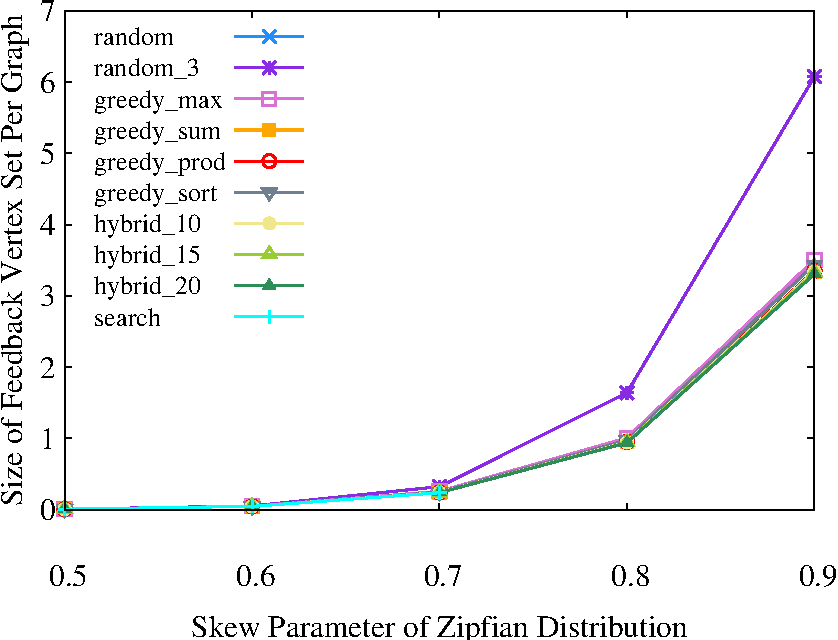
\includegraphics[width=\textwidth]{./exp_fig/fvs/fvs}
        \vspace{-2em}
        \caption{Size of FVS per graph with different algorithms}
        \label{fig:fvs:fvs}
    \end{minipage}
    \begin{minipage}[b]{0.32\linewidth}
        \centering
        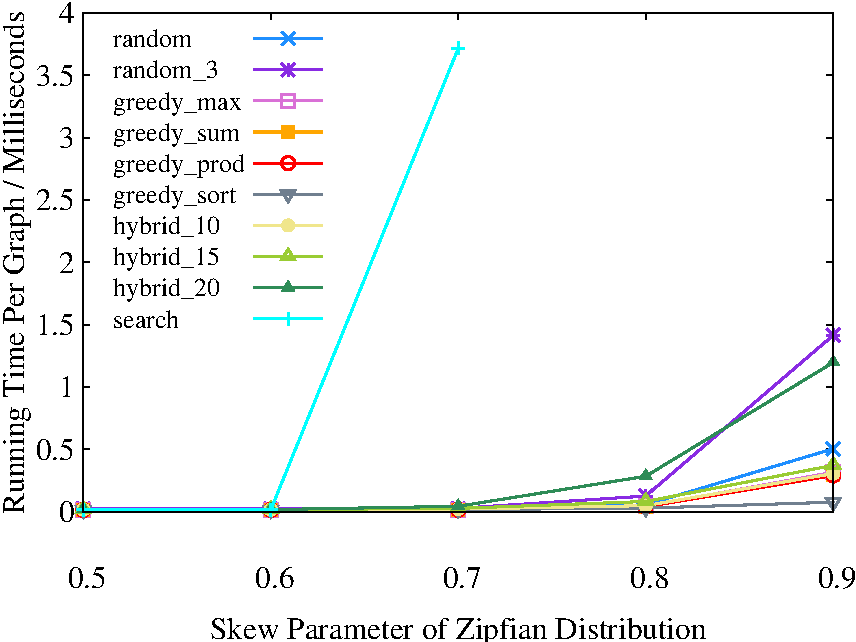
\includegraphics[width=\textwidth]{./exp_fig/fvs/latency}
        \vspace{-2em}
        \caption{Running time of finding FVS with different algorithms}
        \label{fig:fvs:latency}
    \end{minipage}
    \begin{minipage}[b]{0.32\linewidth}
        \centering
        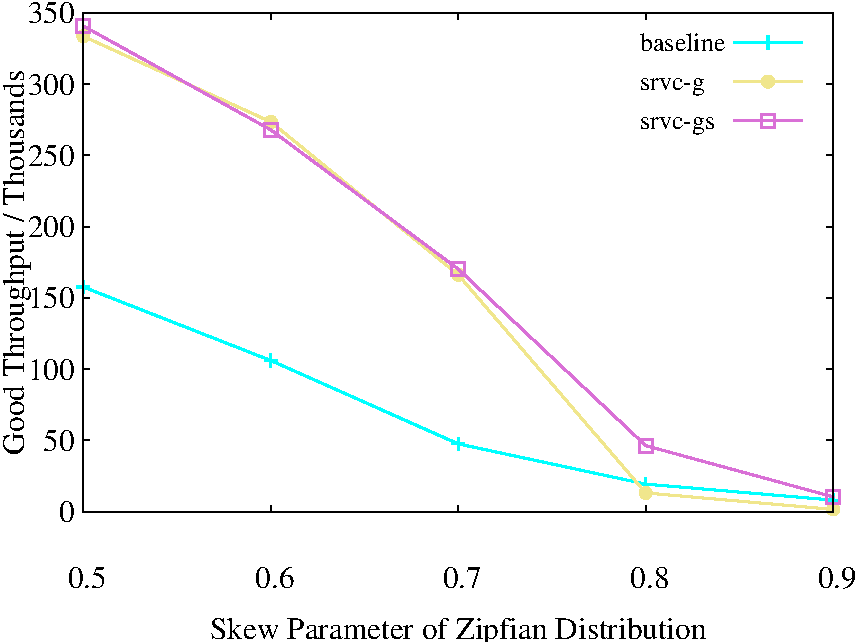
\includegraphics[width=\textwidth]{./exp_fig/fvs/tps}
        \vspace{-2em}
        \caption{Throughput with SCC-based and sort-based greedy algorithms}
        \label{fig:fvs:tps}
    \end{minipage}
    \vspace{-1em}
\end{figure*}

\begin{figure*}[t]
    \centering
    \begin{minipage}[b]{0.32\linewidth}
        \centering
        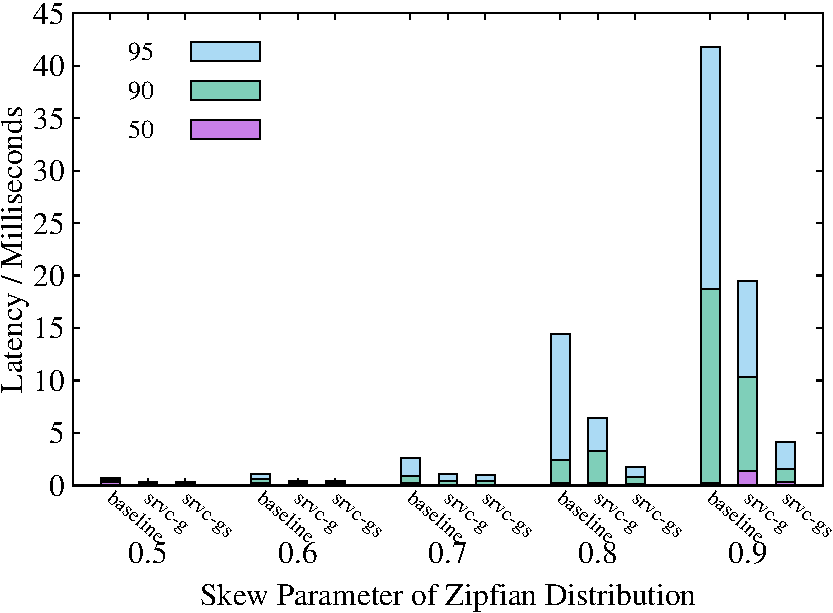
\includegraphics[width=\textwidth]{./exp_fig/fvs/percent95_latency}
        \vspace{-2em}
        \caption{Percentile latency for greedy algorithms}
        \label{fig:fvs:p95}
    \end{minipage}
    \begin{minipage}[b]{0.32\linewidth}
            \centering
            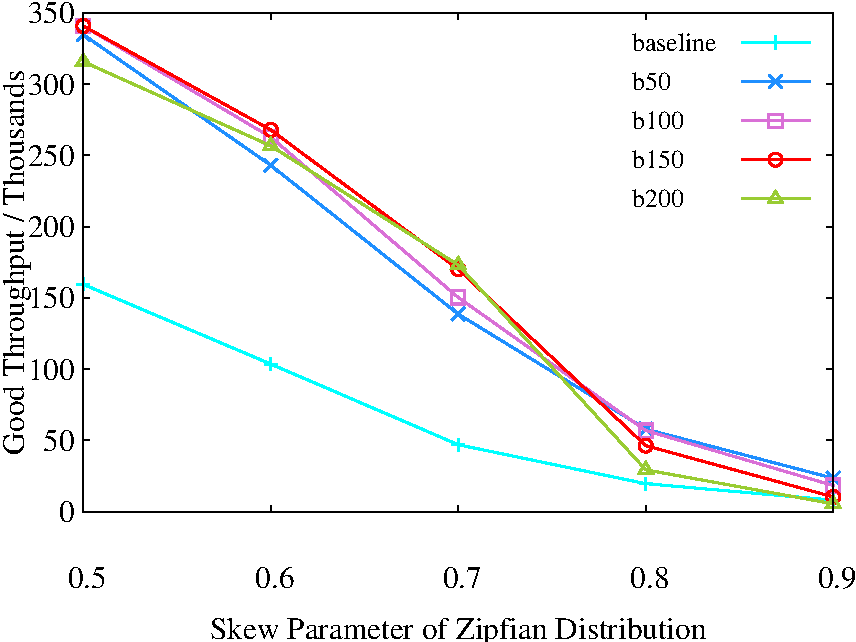
\includegraphics[width=\textwidth]{./exp_fig/bsize/tps}
            \vspace{-2em}
            \caption{Throughput with various batch sizes}
            \label{fig:bsize:tps}
        \end{minipage}
    \begin{minipage}[b]{0.32\linewidth}
        \centering
        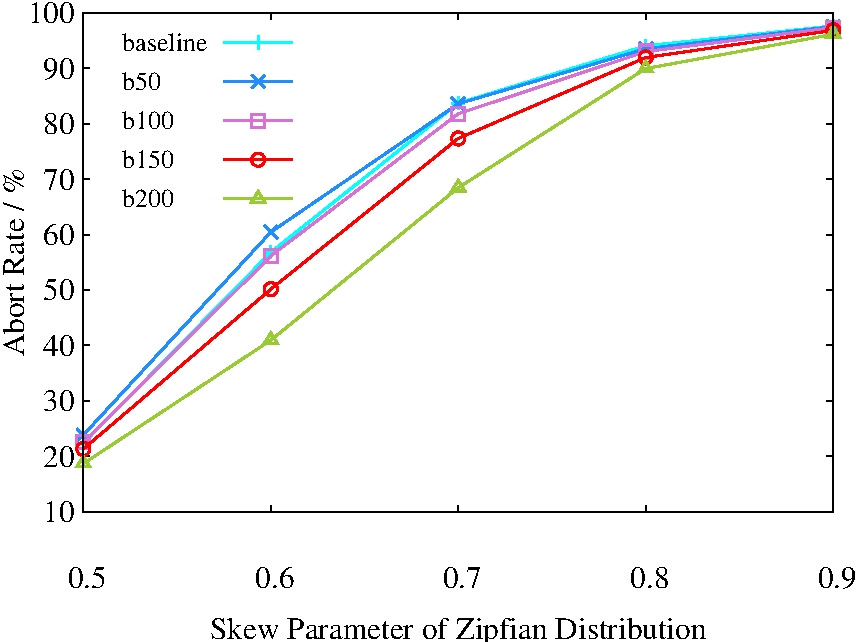
\includegraphics[width=\textwidth]{./exp_fig/bsize/abort}
        \vspace{-2em}
        \caption{Abort rate with various batch sizes}
        \label{fig:bsize:abort}
    \end{minipage}
    \vspace{-1em}
\end{figure*}

\begin{figure*}[t]
    \centering
    \begin{minipage}[b]{0.32\linewidth}
        \centering
        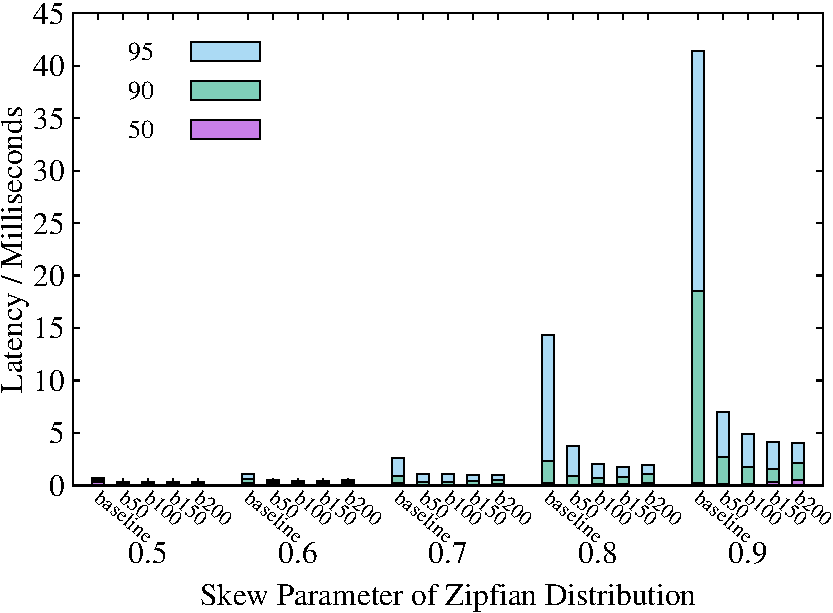
\includegraphics[width=\textwidth]{./exp_fig/bsize/percent95_latency}
        \vspace{-2em}
        \caption{Percentile latency with various batch sizes}
        \label{fig:bsize:p95}
    \end{minipage}
    \begin{minipage}[b]{0.32\linewidth}
            \centering
            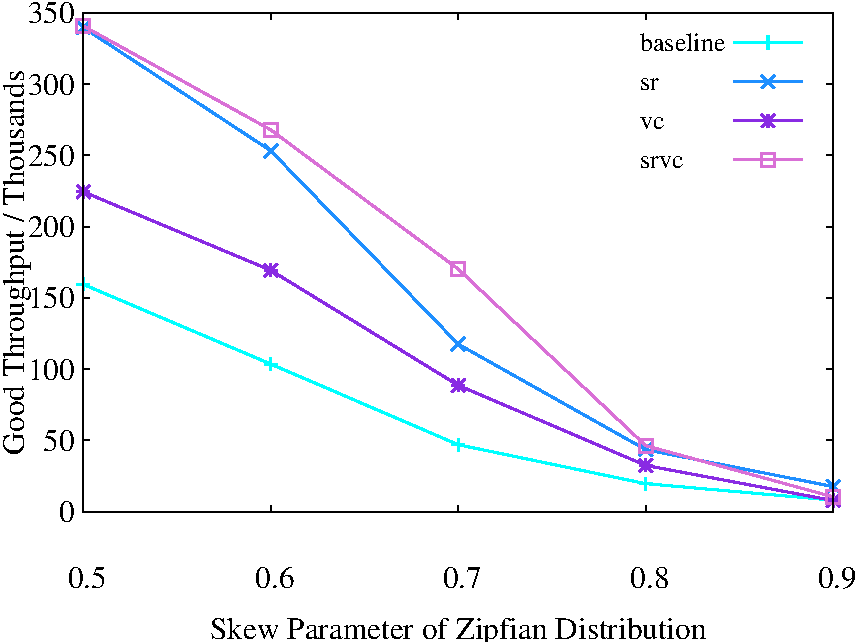
\includegraphics[width=\textwidth]{./exp_fig/basic/tps}
            \vspace{-2em}
            \caption{Throughput under workloads of Zipfian distribution}
            \label{fig:basic:tps}
        \end{minipage}    
    \begin{minipage}[b]{0.32\linewidth}
        \centering
        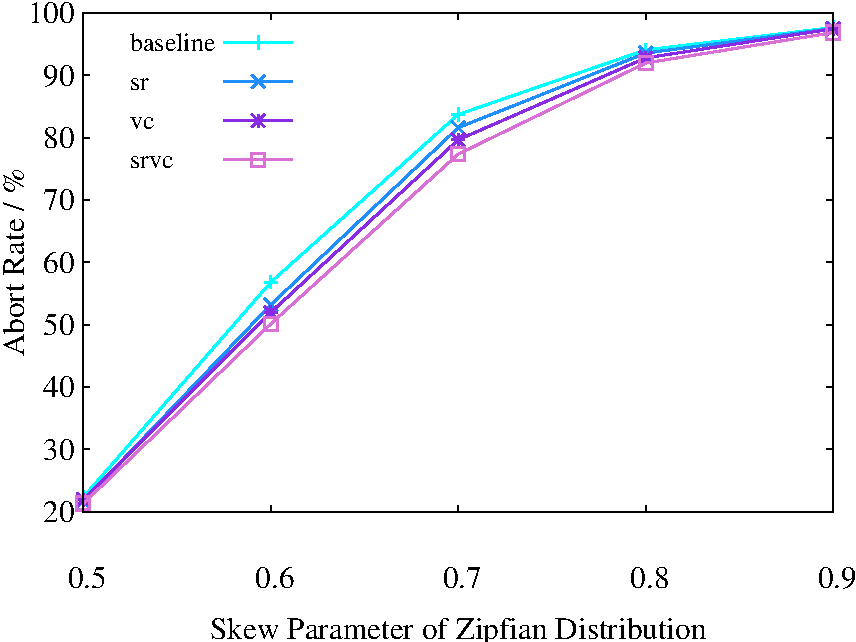
\includegraphics[width=\textwidth]{./exp_fig/basic/abort}
        \vspace{-2em}
        \caption{Abort rate under workloads of Zipfian distribution}
        \label{fig:basic:abort}
    \end{minipage}
    \vspace{-1em}
\end{figure*}

\begin{figure*}[t]
    \centering
    \begin{minipage}[b]{0.32\linewidth}
        \centering
        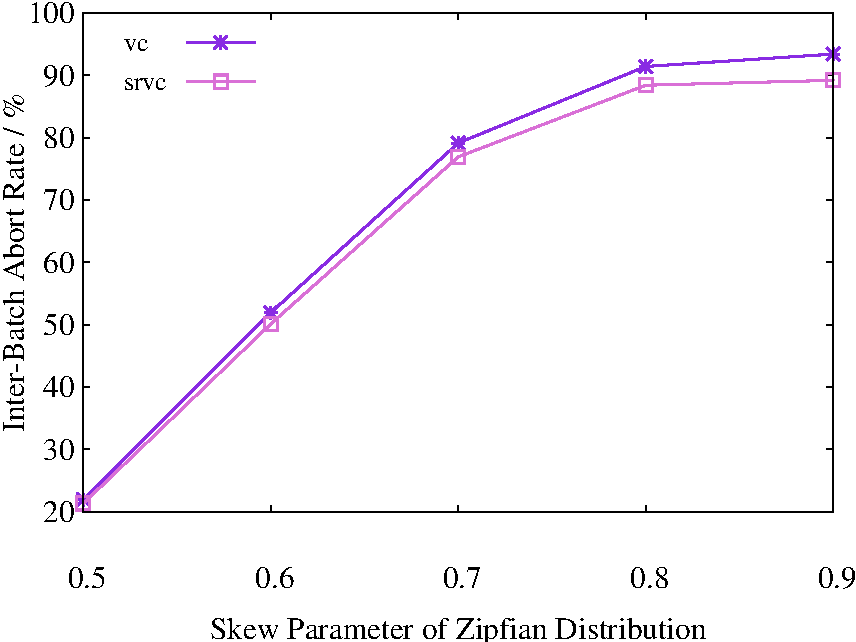
\includegraphics[width=\textwidth]{./exp_fig/basic/preabort}
        \vspace{-2em}
        \caption{Inter-batch aborts under workloads of Zipfian distribution}
        \label{fig:basic:preabort}
    \end{minipage}
    \begin{minipage}[b]{0.32\linewidth}
        \centering
        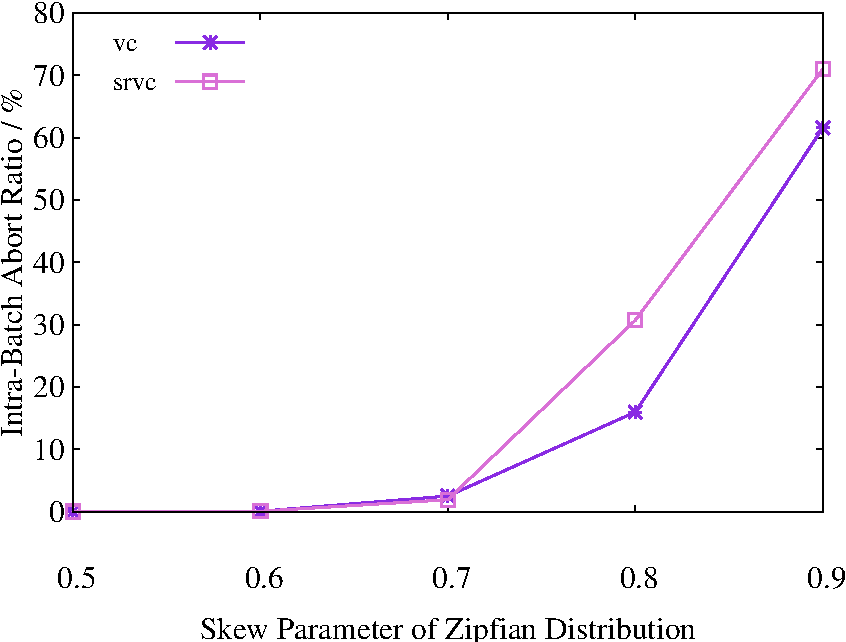
\includegraphics[width=\textwidth]{./exp_fig/basic/in_batch_abort}
        \vspace{-2em}
        \caption{Intra-batch aborts under workloads of Zipfian distribution}
        \label{fig:basic:in_batch_abort}
    \end{minipage}
    \begin{minipage}[b]{0.32\linewidth}
        \centering
        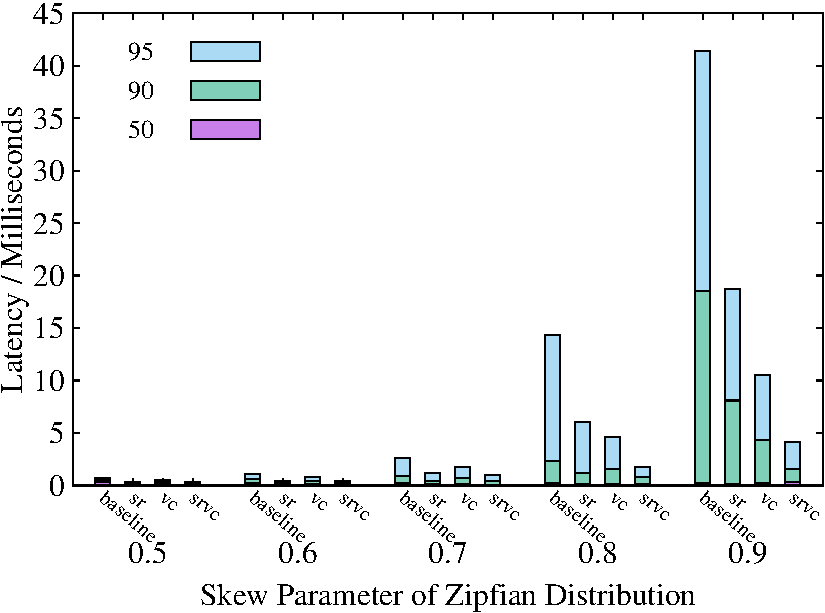
\includegraphics[width=\textwidth]{./exp_fig/basic/percent95_latency}
        \vspace{-2em}
        \caption{Percentile latency under workloads of Zipfian distribution}
        \label{fig:basic:p95}
    \end{minipage}
    \vspace{-1em}
\end{figure*}

\begin{figure*}[t]
    \centering
    \begin{minipage}[b]{0.32\linewidth}
        \centering
        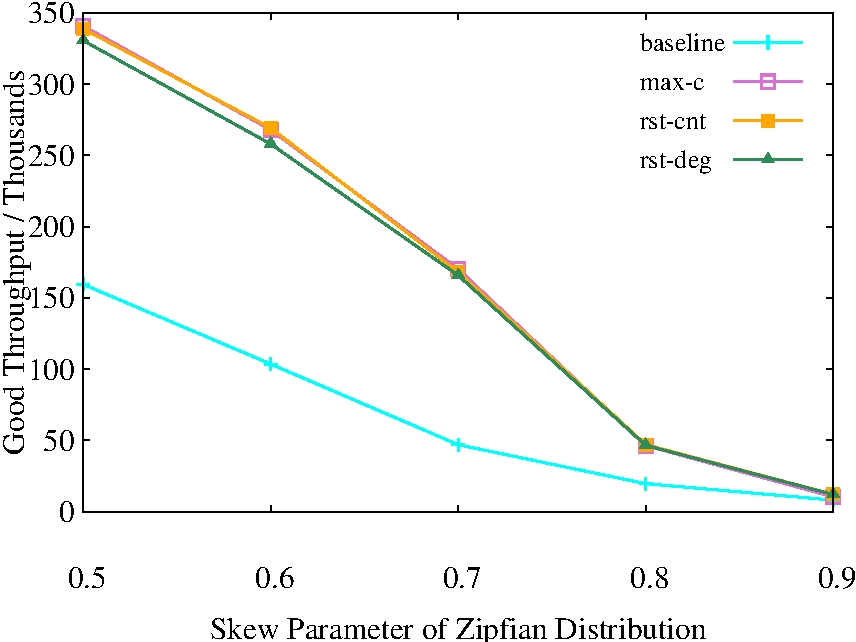
\includegraphics[width=\textwidth]{./exp_fig/restart/tps}
        \vspace{-2em}
        \caption{Throughput with tail latency optimized policies}
        \label{fig:restart:tps}
    \end{minipage}
    \begin{minipage}[b]{0.32\linewidth}
        \centering
        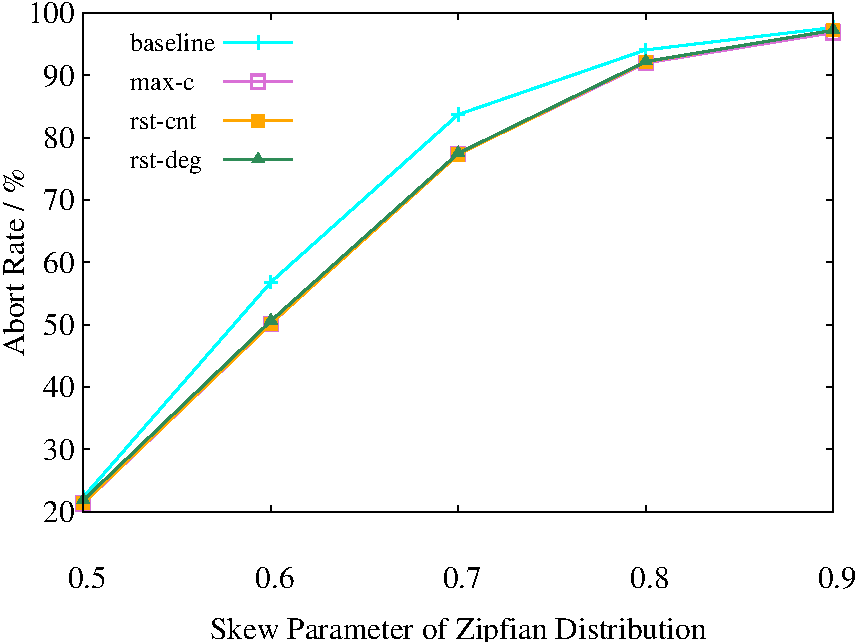
\includegraphics[width=\textwidth]{./exp_fig/restart/abort}
        \vspace{-2em}
        \caption{Abort rate with tail latency optimized policies}
        \label{fig:restart:abort}
    \end{minipage}
    \begin{minipage}[b]{0.32\linewidth}
            \centering
            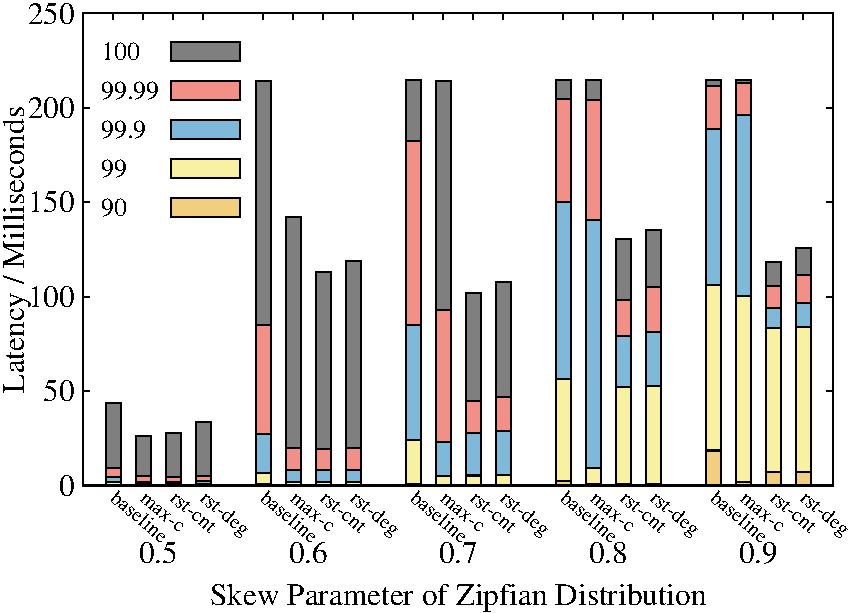
\includegraphics[width=\textwidth]{./exp_fig/restart/percent100_latency}
            \vspace{-2em}
            \caption{Percentile latency with tail latency optimized policies}
            \label{fig:restart:p100}
        \end{minipage}
    \vspace{-1em}
\end{figure*}


% hard transactions
\begin{figure*}[t]
    \centering
    \begin{minipage}[b]{0.32\linewidth}
        \centering
        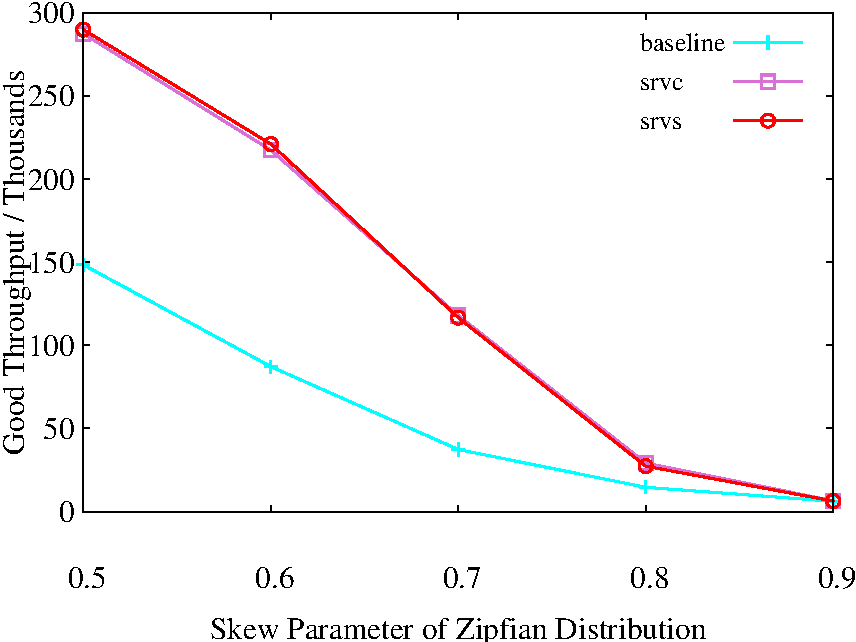
\includegraphics[width=\textwidth]{./exp_fig/weighted_size/tps}
        \vspace{-2em}
        \caption{Throughput with heterogenuous workloads}
        \label{fig:weighted:tps}
    \end{minipage}
\eat{
    \begin{minipage}[b]{0.32\linewidth}
        \centering
        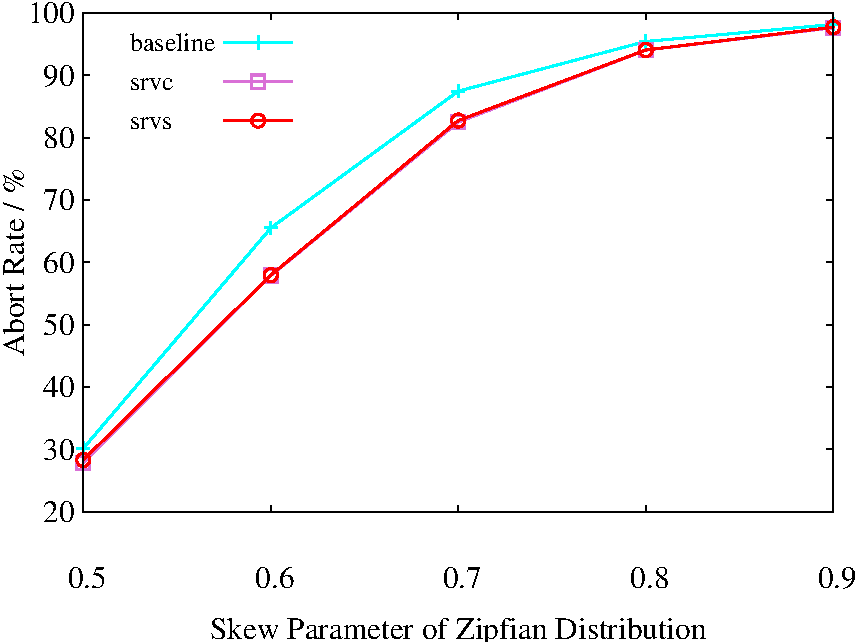
\includegraphics[width=\textwidth]{./exp_fig/weighted_size/abort}
        \vspace{-2em}
        \caption{Abort rate with heterogenuous workloads}
        \label{fig:weighted:abort}
    \end{minipage}
}
    \begin{minipage}[b]{0.32\linewidth}
            \centering
            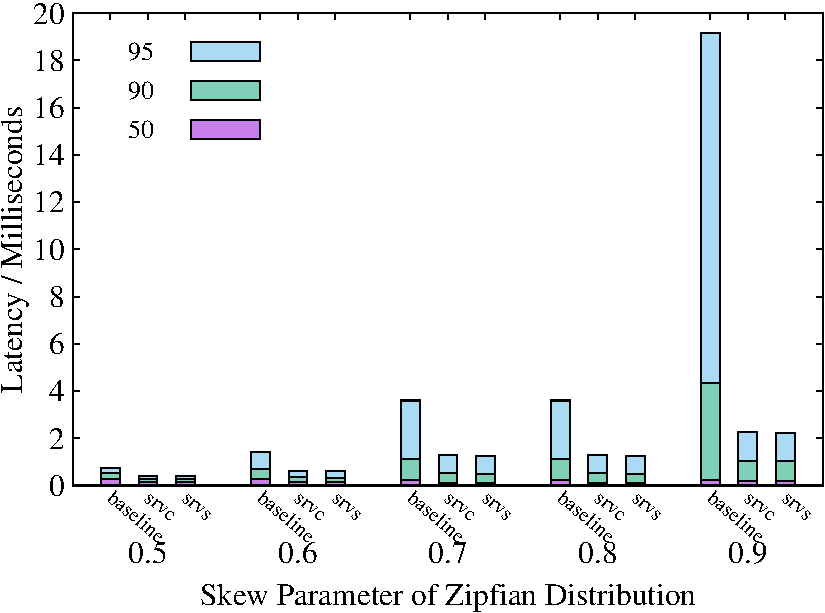
\includegraphics[width=\textwidth]{./exp_fig/weighted_size/percent95_latency}
            \vspace{-2em}
            \caption{Percentile latency with heterogenuous workloads}
            \label{fig:weighted:p95}
        \end{minipage}
        \begin{minipage}[b]{0.32\linewidth}
        \centering
        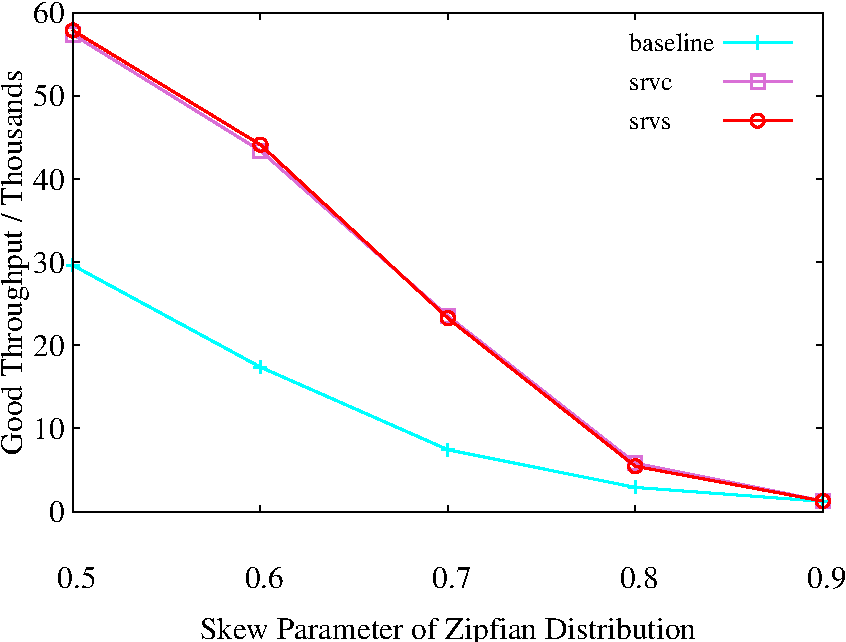
\includegraphics[width=\textwidth]{./exp_fig/weighted_size/tps_1}
        \vspace{-2em}
        \caption{Throughput of large size transactions}
        \label{fig:weighted:tps1}
    \end{minipage}
    \vspace{-1em}
\end{figure*}
\begin{figure*}[t]
    \centering
    \begin{minipage}[b]{0.32\linewidth}
        \centering
        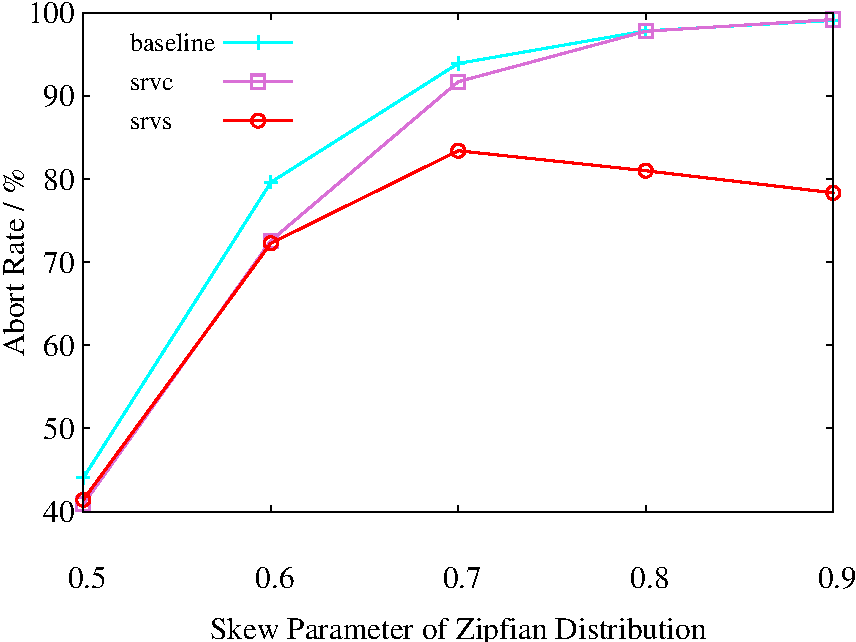
\includegraphics[width=\textwidth]{./exp_fig/weighted_size/abort_1}
        \vspace{-2em}
        \caption{Abort rate of large size transactions}
        \label{fig:weighted:abort1}
    \end{minipage}
    \begin{minipage}[b]{0.32\linewidth}
        \centering
        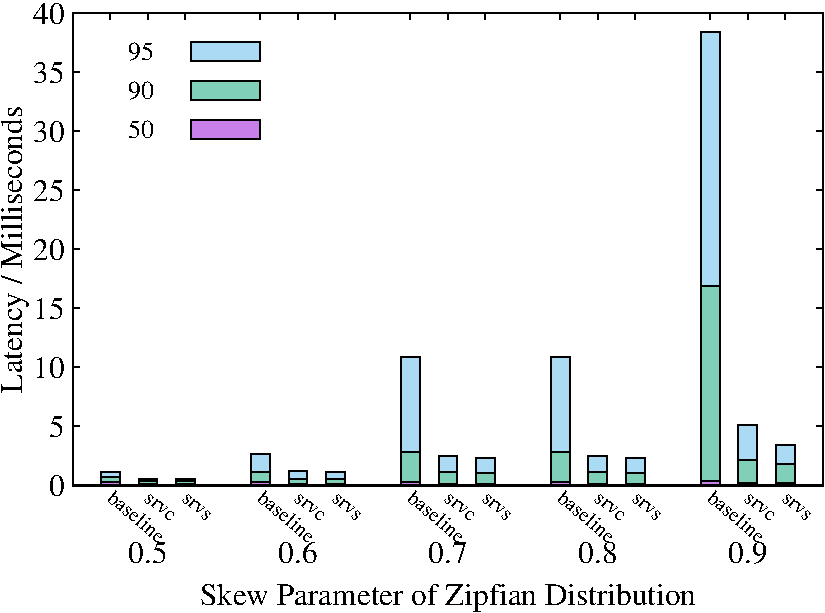
\includegraphics[width=\textwidth]{./exp_fig/weighted_size/percent95_latency_1}
        \vspace{-2em}
        \caption{Percentile latency of large size transactions}
        \label{fig:weighted:p951}
    \end{minipage}
    \begin{minipage}[b]{0.32\linewidth}
        \centering
        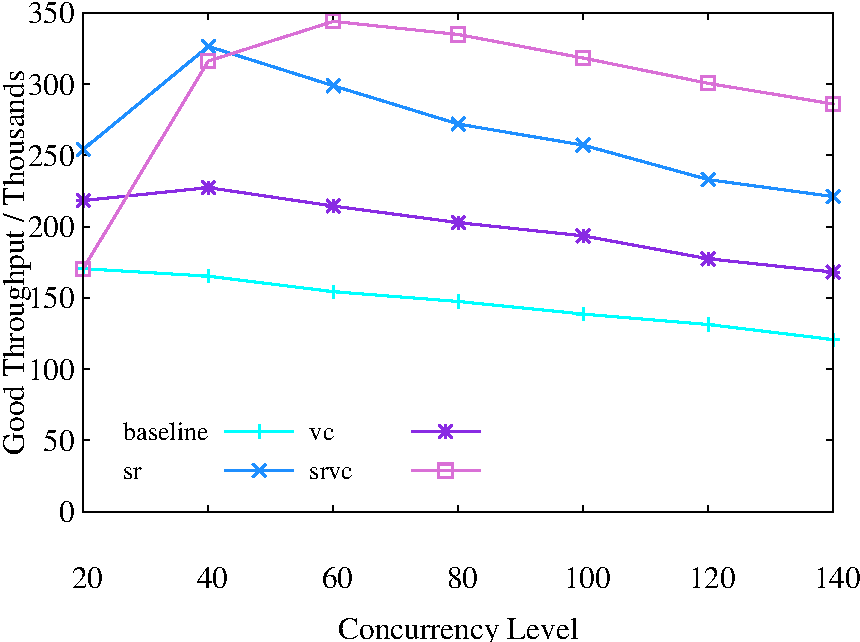
\includegraphics[width=\textwidth]{{{./exp_fig/load/Z0.7.tps}}}
        \vspace{-2em}
        \caption{Throughput with micro benchmark}
        \label{fig:load:tps}
    \end{minipage}
    \vspace{-1em}
\end{figure*}

\begin{figure*}[t]
    \centering
    \begin{minipage}[b]{0.32\linewidth}
      	\centering
        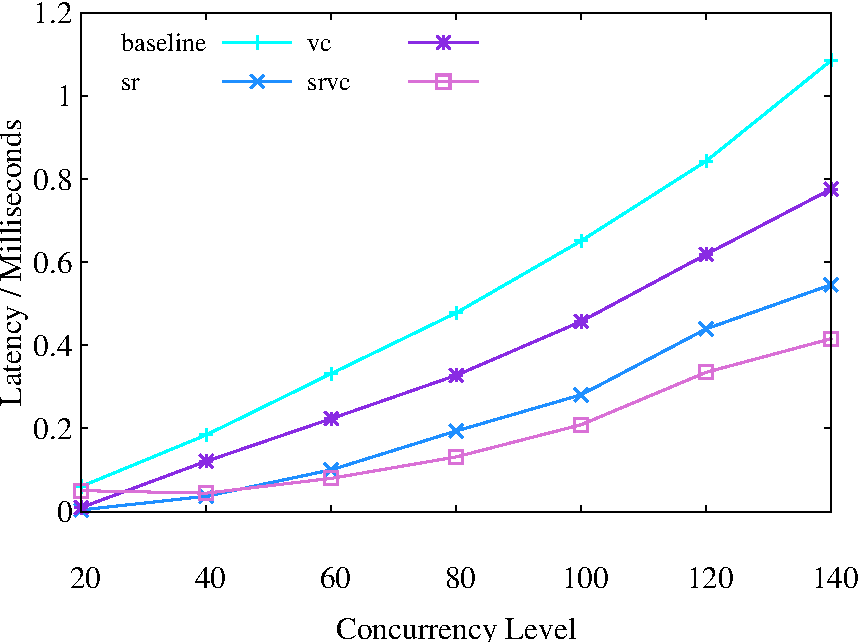
\includegraphics[width=\textwidth]{{{./exp_fig/load/Z0.7.latency}}}
        \vspace{-2em}
        \caption{Average latency with micro benchmark}
        \label{fig:load:latency}
    \end{minipage}
    \begin{minipage}[b]{0.32\linewidth}
        \centering
        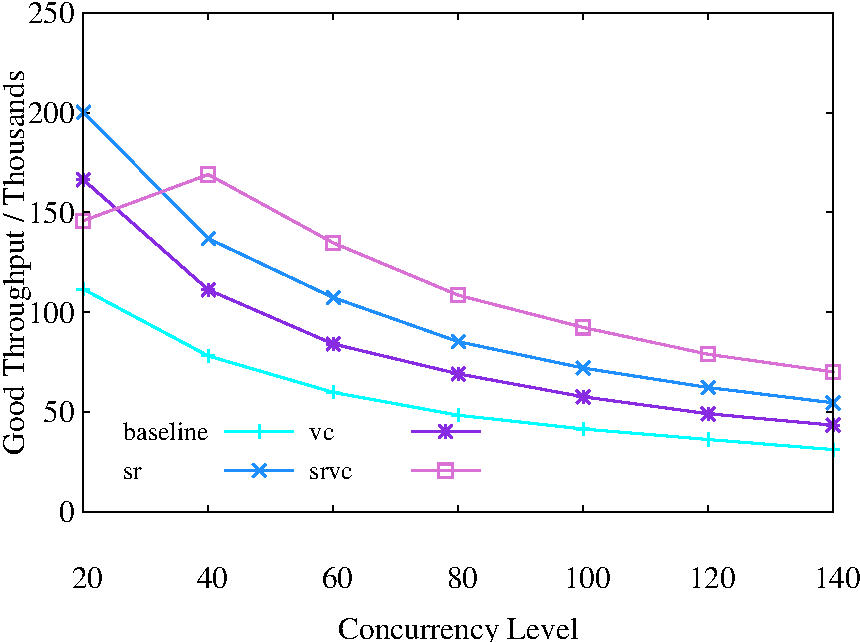
\includegraphics[width=\textwidth]{{{./exp_fig/small_bank/Z0.9.tps}}}
        \vspace{-2em}
        \caption{Throughput with Small Bank benchmark}
        \label{fig:small_bank:tps}
    \end{minipage}
    \begin{minipage}[b]{0.32\linewidth}
        \centering
        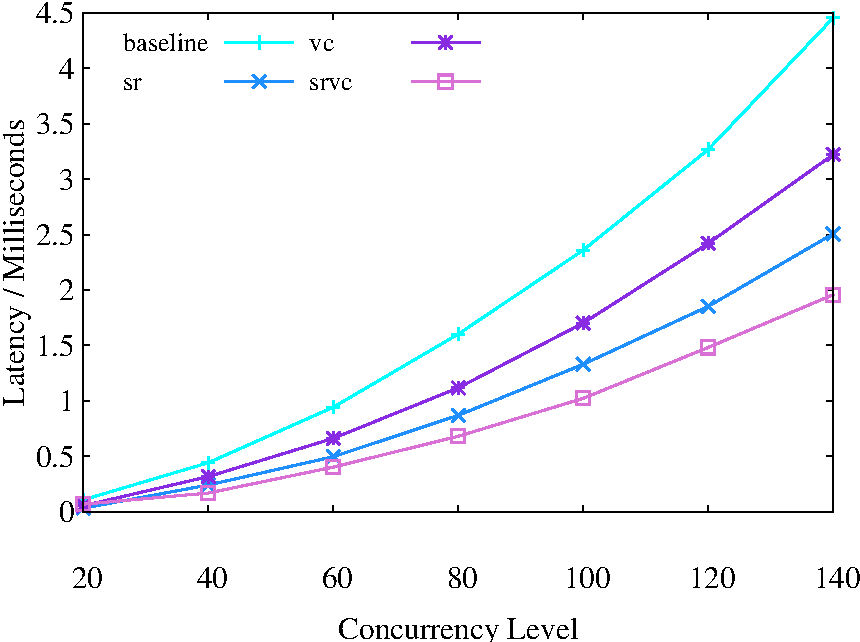
\includegraphics[width=\textwidth]{{{./exp_fig/small_bank/Z0.9.latency}}}
        \vspace{-2em}
        \caption{Average latency with Small Bank benchmark}
        \label{fig:small_bank:latency}
    \end{minipage}
    \vspace{-1em}
\end{figure*}

\subsection{Validator Reordering Algorithms}
In our first experiment, we investigate the performance of the feedback vertex set algorithms from Section~\ref{subsec:validator_reordering:algorithm}. 

We begin with a comparison of the algorithms with respect to their raw performance - i.e., their accuracy and running time. We run the algorithms on graphs constructed as described in Section~\ref{sec:ibvr}, using a variety of workloads generated from a Zipfian distribution. 

We first test the algorithms offline on dependency graphs constructed at the validator when running the system. Each dependency graph is constructed from a batch of transactions at the validator, excluding non-viable transactions, i.e. transactions that have inter-batch conflicts. We compare the averages of the size of the feedback vertex set and the running time per dependency graph on each trace.

We test the SCC-based greedy algorithm with the \texttt{max-degree} ($greedy\_max$), \texttt{sum-degree} ($greedy\_sum$) and \texttt{prod-degree} policies ($greedy\_prod$). We also test the sort-based greedy algorithm $greedy\_sort$ (using the \texttt{prod-degree} policy for sorting and multi factor 2), and the hybrid algorithm $hybrid\_m$. The hybrid algorithm uses $greedy\_prod$ as a subroutine when the size of the SCC is larger than $m$, and switches to the brute force search otherwise. By increasing the threshold, we can progressively approximate the optimal solution. 


We test these algorithms against several baselines. $search$ is an accurate, brute force FVS search algorithm. $random$ is the SCC-based greedy algorithm and removes a vertex at random from each SCC to break the cycle. Our final baseline runs the random algorithm multiple times (3 times for $random\_3$) on each graph, and returns the smallest FVS across all the runs. This mitigates the worst-case impact of bad random choices.


Figure~\ref{fig:fvs:fvs} shows the average size of the feedback vertex set found by each algorithm. The brute force search algorithm is so slow that it cannot produce results once the skew factor increases beyond $0.7$ as the graphs become denser.
The figure shows that the $random$ baseline computes a FVS whose size is almost twice as large as the greedy and the hybrid algorithms. Running the random algorithm multiple times produces similar results. This confirms the theoretical results which show that finding good feedback vertex sets is hard. The greedy algorithms, on the other hand, produce very accurate results. The average size of the feedback vertex set is almost identical to that of the brute force search when the skew factor is no larger than $0.7$, and is very close to the best hybrid algorithm ($hybrid\_20$, i.e. one that uses the brute force search when the size of the SCC is no larger than 20). Among the greedy algorithms, $greedy\_prod$ is consistently the best, although the difference is small.

Figure~\ref{fig:fvs:latency} shows the running time of the algorithms. The running time of the hybrid algorithm depends on the threshold for switching to brute force search. Thus, $hybrid\_20$ and $hybrid\_15$ have a longer running time than other algorithms, while the running time of $hybrid\_10$ is comparable to the SCC-based algorithms. Each of the SCC-based algorithms ($greedy\_max$, $greedy\_sum$, $greedy\_prod$, $random$) has a similar running time. The random algorithm takes slightly longer than the greedy algorithms because it removes more nodes and thus requires more computation. The running time of $random\_3$ is three times that of $random$, since it runs the random algorithm three times. The sort-based greedy algorithm ($greedy\_sort$), while slightly less accurate than the SCC-based greedy algorithms, reduces the running time of these algorithms to 26\%. 

We compare the end-to-end performance of the best SCC-based algorithm ($greedy\_prod$) against the sort-based greedy algorithm. Figure~\ref{fig:fvs:tps} shows the good throughput of the system with $greedy\_prod$ ($srvc\hbox{-}g$) and $greedy\_sort$ ($srvc\hbox{-}gs$). In both cases, storage batching is enabled, and the greedy algorithm policy is set to minimizing the number of conflicts, i.e. the size of the feedback vertex set. The $baseline$ line shows the throughput with both storage and validator batching disabled. 

The two greedy algorithms have similar throughput when the skew is moderate. However,  $greedy\_prod$ degrades significantly with high data contention (skew factor $0.8$ and $0.9$). This is because while $greedy\_prod$ is slightly more accurate, it takes much longer to run. This increases transaction latency and leads to more aborts, especially when the chance of conflicts is high. $greedy\_sort$ consistently gives the highest throughput over all the workloads, due to its high accuracy and low running time. 

Figure~\ref{fig:fvs:p95} shows transaction latencies by percentile. The percentile latency of $greedy\_sort$ is much lower than that of the baseline and $greedy\_prod$. This is consistent with the throughput data we have seen.

In summary, the sort-based greedy algorithm is much faster than the ``smarter'' algorithms and only slightly worse in terms of accuracy. This means it gives the best end-to-end system performance. For this reason, all subsequent experiments use the sort-based greedy algorithm with a \texttt{prod-degree} policy unless otherwise specified.


\subsection{Batch Size}

In this experiment, we explore how the batch size affects system performance. 
Smaller batch sizes should give lower latencies but they offer fewer opportunities for reordering, leading to more aborts. 

We configure the system to perform both storage and validator batching with batch sizes from $50$ to $200$ ($b50$, $b100$, $b150$, $b200$), using the same batch size at the storage and the validator. As before, $baseline$ is the system with both kinds of batching turned off. 

As expected, increasing the batch size always reduces the number of aborts due to more opportunities for reordering as shown in Figure~\ref{fig:bsize:abort}. 

Figure~\ref{fig:bsize:tps} shows the throughput of the system with different batch sizes as data skew increases. As expected, the throughput first rises as we increase the size of the batch, and then degrades when the batch becomes too large.
\eat{Thus, the throughput with batch size 150 is higher than with batch size 200. }
The percentile latency displays a similar pattern, as shown in Figure~\ref{fig:bsize:p95}. Again the best batch size is 150; however, using batching always gives higher throughput and a better latency profile than the baseline.


Given the above results, a batch size of 150 appears optimal for our configuration; we use this batch size in the remainder of our experiments. 

\subsection{Storage and Validator Batching}
\label{subsec:experiment:batching}

Next, we perform a detailed analysis of the effects of storage and validator batching. We configure the system in several different modes: no batching ($baseline$), storage batching ($sr$), validator batching with the \texttt{prod-degree} policy that maximizes the number of commits ($vc$), and both storage and validator batching ($srvc$).


As explained in Section~\ref{sec:overview}, batching and reordering affect the abort rate by reducing inter-batch and intra-batch aborts. The number of inter-batch aborts is affected by system-wide transaction latency, the freshness of the transactions' reads, and their access patterns. Validator reordering reduces the number of intra-batch aborts; however, storage reordering can increase the number of such aborts because it reduces inter-batch aborts (and thus more viable transactions end up in validator batches rather than aborting due to inter-batch conflicts). The overall good throughput of the system is affected by both the transaction latency and the abort rate. 


Figure~\ref{fig:basic:tps}, Figure~\ref{fig:basic:abort}, and Figure~\ref{fig:basic:p95} show the good throughput, the abort rate, and the percentile latency of different system modes under a variety of data skew parameters. Figure~\ref{fig:basic:preabort} shows the percent of inter-batch aborts, while Figure~\ref{fig:basic:in_batch_abort} shows the intra-batch abort ratio, i.e. the number of transactions that commit divided by the number of viable transactions in a batch.


Overall, using batching at the storage and/or the validator consistently leads to significant improvements in throughput, abort rate, and latency profiles over the baseline. When batching is enabled ($sr$ and $srvc$), the throughput is 2.1x-3.7x that of the baseline ($baseline$). In addition, using validator batching always reduces the abort rate, as shown in Figure~\ref{fig:basic:abort}, and gives a better latency profile (Figure~\ref{fig:basic:p95}).

When the data contention is very low\eat{, i.e. when the skew factor is 0.5}, the abort rate is low (Figure~\ref{fig:basic:abort}). In addition, the abort rate is dominated by inter-batch conflicts (Figure~\ref{fig:basic:preabort}) and intra-batch conflicts are rare (Figure~\ref{fig:basic:in_batch_abort}). Thus, the storage-batching-only mode ($sr$) gives similar throughput as with $srvc$.  As the data skew increases, so does the number of intra-batch conflicts and aborts; the overhead of validator batching starts to pay off. In a medium-contention setting, using both validator and storage batching ($srvc$) gives the best throughput. When the data contention is extremely high\eat{, i.e. the skew factor reaches 0.9}, the number of intra-batch conflicts that cannot be resolved by validator reordering increases. The validator reordering takes more time due to denser graphs, while bringing less benefit. Thus, the best throughput is achieved by using storage batching only ($sr$). 

To summarize, it is always beneficial to enable storage batching since this technique reduces inter-batch aborts at a minimal cost. While validator batching consistently gives a better abort rate and percentile latency, it is most effective in mid-contention settings, when the reduction of intra-batch conflicts that it brings is sufficient to justify its cost. 

\subsection{More Policies for Validator Reordering}

In the next set of experiments, we explore validator reordering with the more complex policies presented in Section~\ref{subsec:validator_reordering:policy}; specifically, we look at policies that aim to reduce the transaction tail latency, and at policies that help ``hard transactions'' with many dependencies commit.


\subsubsection{Reducing tail latencies}

We explore the possibility of reducing transaction tail latency with latency-specific policies. Our baselines are the \texttt{prod-degree} policy that maximizes the number of commits ($max\hbox{-}c$) as well as the $baseline$ with no batching. 

Our first tail-latency aware policy ($rst\hbox{-}cnt$) favors transactions that have already been aborted and restarted. When choosing a node to include in the feedback vertex set, it chooses the one with the smallest number of restarts, breaking ties using \texttt{prod-degree}.

The second latency-aware policy considers both the number of restarts and a degree-based measurement of a transaction. It computes the weight of a node as the product of in-degree and out-degree over the exponential of the number of restarts with base 2. When choosing a node to include in the feedback vertex set, the nodes are sorted in descending order by their weights. Thus, a node with a high degree product can have its weight reduced if the corresponding transaction has restarted many times.

Figure~\ref{fig:restart:tps} and Figure~\ref{fig:restart:abort} show the transaction throughput and abort rate. As expected, the impact of tail-latency aware policies on overall transaction policies is slightly worse than the \texttt{prod-degree} policy due to its suboptimality in finding the minimal feedback vertex set.

Figure~\ref{fig:restart:p100} shows the tail latency from 90\% to 100\%, i.e. the latency threshold for up to 90\% and up to 100\% of the transactions. While maximizing the number of commits, the \texttt{prod-degree} policy can produce worse tail latencies than the baseline. This is because it is unaware of the restart times of transactions, and it can discriminate against transactions that are inherently hard to commit, e.g. because they access many hot items.

In contrast, the latency-aware policies $rst\hbox{-}cnt$ and $rst\hbox{-}deg$ have similar overall performance profiles and consistently perform significantly better than $baseline$ and the $max\hbox{-}c$, especially for tail latencies from 99.9\% to 100\%.  \eat{, although $rst\hbox{-}deg$ consistently performs slightly better than $rst\hbox{-}cnt$.}

In summary, the latency-aware policies decrease tail latencies significantly while maintaining a comparable overall performance to the policy that maximizes the number of commits. Moreover, a simple latency-aware policy that privileges the number of restarts over the graph degree is as effective as a more sophisticated policy that combines the graph degree and the number of restarts together.


\subsubsection{Helping hard transactions commit}

We simulate a heterogeneous workload by including 80\% of normal transactions with 5 reads and 5 writes, and 20\% of ``hard transactions'' with 10 reads and 10 writes. All the data accesses are drawn from the same Zipfian distribution. The larger transactions are more likely to conflict with others and less likely to commit; thus, we assign them higher priorities in the validator reordering. We compare the system performance with unweighted ($srvc$) validator reordering and a weighted ($srvs$) validator reordering policy that privileges the larger transactions. In both cases, storage batching is enabled. As before, the $baseline$ configuration uses no batching.

Figures~\ref{fig:weighted:tps} and~\ref{fig:weighted:p95} show the overall throughput and the percentile latency. Since the ratio of large transactions is small, the overall performance under weighted and unweighted reordering policies is similar.

Figures~\ref{fig:weighted:tps1},~\ref{fig:weighted:abort1}, and~\ref{fig:weighted:p951} show the throughput, the abort rate, and the percentile latency of the larger transactions alone. While the throughput of unweighted and weighted validator reordering is still similar, weighted validator reordering gives a much better transaction profile as far as the abort rate and the percentile latency are concerned.

\subsection{End-to-End Performance on Benchmarks}
\label{subsec:experiment:end2end}
In our final experiment, we explore the end-to-end performance of batching in a realistic setting where batch size is fixed. We use two workloads: a micro benchmark and the Small Bank benchmark~\cite{alomari2008icde}. In our micro benchmark,  we generate the transactions as described in Section~\ref{subsec:experiment:implementation}. \eat{We introduce skewed accesses to the data where each item is drawn from Zipfian distribution.} The Small Bank benchmark contains transactions with a realistic and diverse combination of read and write conflicts. The transactions come from the financial domain: compute the balance of a customer's checking and savings accounts, deposit money to a checking account, transfer money from a checking account to a savings account, move all funds from one customer to another customer, and withdraw money from a customer's account. We use a Zipfian distribution to simulate skewed data accesses. We populate the database with 100K customers, i.e. 100K checking and 100K savings accounts. We use a batch size of 10 transactions and we vary the system concurrency level from 20 to 140 transactions. We simulate high data contention by introducing Zipfian skew factor (0.7 for the micro benchmark and 0.9 for the Small Bank benchmark, which has shorter transactions).
\eat{, i.e. the limit of active transactions in the system}


\eat{On the micro benchmark, Figure~\ref{fig:load:tps} shows the throughput at skew factor 0.7.} 
On the micro benchmark, Figure~\ref{fig:load:tps} shows the throughput. 
Using batching doubles the throughput as compared to the baseline, both for a given load and when considering the peak throughput over different loads. When the load is moderate, storage batching by itself performs best. As the load increases and the transactions become more conflict-prone, the benefit of validator batching outweighs its cost. This confirms our observation in Section~\ref{subsec:experiment:batching}. 

Figure~\ref{fig:load:latency} shows the average transaction latency. Both storage and validator batching reduce the latency as compared to the baseline. In addition, validator batching always reduces latency regardless of whether storage batching is enabled, again confirming our findings in Section~\ref{subsec:experiment:batching}.

\eat{Figures~\ref{fig:small_bank:tps} and~\ref{fig:small_bank:latency} show the throughput and latency of the system on the Small Bank benchmark at skew factor 0.9. }
Figures~\ref{fig:small_bank:tps} and~\ref{fig:small_bank:latency} show the throughput and latency of the system on the Small Bank benchmark. 
The performance impacts of batching are similar to those on the micro benchmark.

We ran additional experiments on both benchmarks varying the data skew; results were similar to those shown and are omitted due to space limitations.
